\documentclass[journal,12pt,twocolumn]{IEEEtran}
\usepackage{cite}
\usepackage{amsmath,amssymb,amsfonts,amsthm}
\usepackage{graphicx}
\title{GATE-2023 EC Q.25}
\author{EE23BTECH11214 - Harsha Vardhan Kumar}

\begin{document}
\maketitle

\textbf{Question}:
In the context of signals and systems, determine the phase cross-over frequency of the open-loop transfer function
\[
G(s) = \frac{k \cdot s \cdot (1+sT_1) \cdot (1+sT_2)}{s}
\]
with positive constants $k, T_1, T_2$ are positive constants.The phase crossover fequency,in rad/s,is
\hfill [EC,GATE-$2023$]
\begin{enumerate}
  \item[(a)] $\frac{1}{\sqrt{T_1 T_2}}$
  \item[(b)] $\frac{1}{T_1 T_2}$
  \item[(c)] $\frac{1}{T_1\sqrt{T_2}}$
  \item[(d)] $\frac{1}{\sqrt{T_2}T_1}$
\end{enumerate}
\textbf{Solution}:
The phase of \( G(s) \)
\begin{align}
\angle G(s) &= \angle (ks(1+sT_1)(1+sT_2)) - \angle s \\
&= \angle ks + \angle (1+sT_1) + \angle (1+sT_2) - \angle s 
\end{align}
The phase contribution of each term
\begin{align}
\angle ks &= \angle k + \angle s = 0 + \frac{\pi}{2} \\
&= \frac{\pi}{2} \text{ radians} \\
\angle (1+sT_1) &= \tan^{-1}(0) + \tan^{-1}(sT_1) \\
&= \tan^{-1}(sT_1)  \\
\angle (1+sT_2) &= \tan^{-1}(0) + \tan^{-1}(sT_2)\\ 
&= \tan^{-1}(sT_2)  \\
\angle s &= \frac{\pi}{2} \text{ radians} 
\end{align}

So, the total phase of \( G(s) \) becomes:
\begin{align}
\angle G(s) &= \frac{\pi}{2} + \tan^{-1}(sT_1) + \tan^{-1}(sT_2) - \frac{\pi}{2}  \\
&= \tan^{-1}(sT_1) + \tan^{-1}(sT_2)
\end{align}

the frequency at which the phase angle \( \angle G(s) \) equals \( -\pi \) radians.

\begin{align}
\tan^{-1}(j\omega T_1) + \tan^{-1}(j\omega T_2) &= -\pi \\
\tan^{-1}(j\omega T_1) + \tan^{-1}(j\omega T_2) &= -\frac{\pi}{2} \\
\tan^{-1}(j\omega T_1) &= -\frac{\pi}{2} - \tan^{-1}(j\omega T_2) \\
j\omega T_1 &= \tan\left(-\frac{\pi}{2} - \tan^{-1}(j\omega T_2)\right) \\
j\omega T_1 &= -\frac{1}{\tan(\tan^{-1}(j\omega T_2))} \\
j\omega T_1 &= -\frac{1}{j\omega T_2} \\
\omega T_1 &= \frac{1}{\omega T_2} \\
\omega^2 &= \frac{1}{T_1 T_2} \\
\omega &= \frac{1}{\sqrt{T_1 T_2}}
\end{align}

the phase cross-over frequency is \[ {\frac{1}{\sqrt{T_1 T_2}}} \]
\begin{figure}[!ht] 
\centering
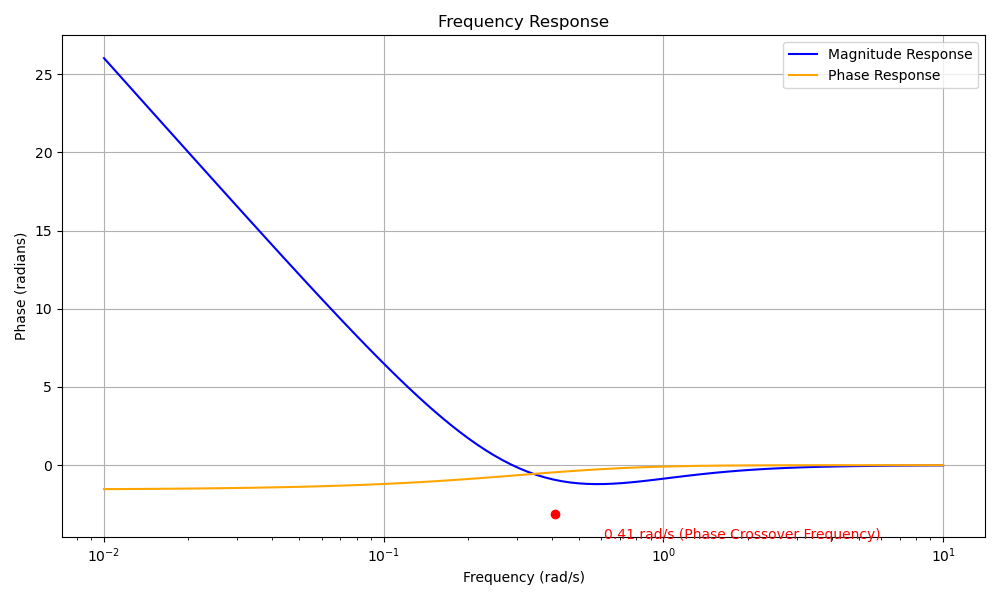
\includegraphics[width=2\columnwidth]{graph.png}
\label{fig:Graph1}
\end{figure}
\end{document}
